




\begin{figure}
    \centering
    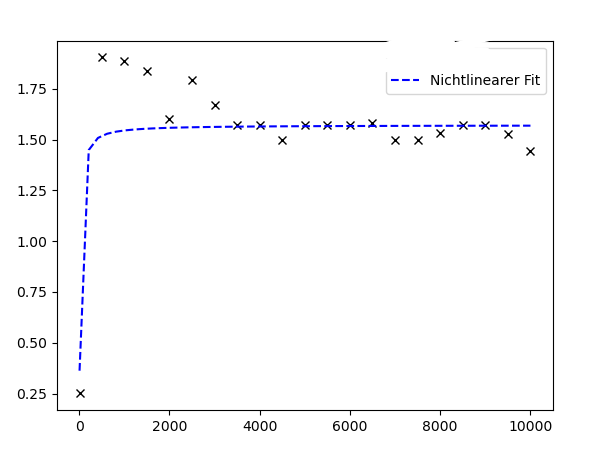
\includegraphics[width=0.5\textwidth]{build/plot1.pdf}
    \caption{Graphische Darstellung der annährend linearen Werte aus der Messrehe der Wellenlänge $\lambda = 546 [\si{\nano\meter}]$ mit eingeszeichneter linearen Ausgleichsgerade.} 
    \label{fig:müdes}
\end{figure}

\begin{figure}
    \centering
    \includegraphics[width=0.5\textwidth]{build/plot2.pdf}
    \caption{Graphische Darstellung der annährend linearen Werte aus der Messrehe der Wellenlänge $\lambda = 546 [\si{\nano\meter}]$ mit eingeszeichneter linearen Ausgleichsgerade.} 
    \label{fig:grün}
\end{figure}

\begin{figure}
    \centering
    \includegraphics[width=0.5\textwidth]{build/plot3.pdf}
    \caption{Graphische Darstellung der annährend linearen Werte aus der Messrehe der Wellenlänge $\lambda = 434,435,436 [\si{\nano\meter}]$ mit eingeszeichneter linearen Ausgleichsgerade.} 
    \label{fig:violet}
\end{figure}

\begin{figure}
    \centering
    \includegraphics[width=0.5\textwidth]{build/plot4.pdf}
    \caption{Graphische Darstellung der annährend linearen Werte aus der Messrehe der Wellenlänge $\lambda = 408,405 [\si{\nano\meter}]$ mit eingeszeichneter linearen Ausgleichsgerade.} 
    \label{fig:GIGAviolet}
\end{figure}







\begin{table}
    \centering
    \caption{Messdaten des Photonenstrom $I_{Phasenstrom}$ bei einer Wellenlänge von $\SI{577}{\nano\meter}$, $\SI{579}{\nano\meter}$ mit einem Spannungsintervall von $\{\SI{-20}{\volt},... ,\SI{20}{\volt}\}$.}
    \label{tab:tab1}
    \begin{tabular}{c c || c c}
        \toprule
        $I_{Phasenstrom}[\si{\nano\ampere}]$ & $U [\si{\volt}] < 0$ & $I_{Phasenstrom}[\si{\nano\ampere}]$ & $U [\si{\volt}] > 0$ \\
        \midrule
        2.60         &         -19.14  &  0            &           0.10    \\    
        2.50         &         -18.00  &  0            &           0.20    \\    
        2.45         &         -16.00  &  0            &           0.30    \\    
        2.40         &         -14.01  &  0            &           0.40    \\    
        2.30         &         -12.02  &  0            &           0.50    \\    
        2.20         &         -10.01  &  0            &           0.60    \\    
        2.09         &         -09.02  &  0            &           0.70    \\    
        2.05         &         -08.02  &  0            &           0.80    \\    
        2.00         &         -07.01  &  0            &           0.90    \\    
        1.81         &         -06.00  &  0            &           1.00    \\    
        1.75         &         -04.98  &  0            &           1.20    \\    
        1.55         &         -04.00  &  -0.001       &           1.40    \\    
        1.30         &         -02.99  &  -0.002       &           1.60    \\    
        1.00         &         -01.99  &  -0.003       &           1.80    \\    
        0.89         &         -01.80  &  -0.004       &           2.00    \\    
        0.82         &         -01.60  &  -0.008       &           3.00    \\    
        0.75         &         -01.40  &  -0.010       &           4.00    \\    
        0.70         &         -01.20  &  -0.014       &           5.00    \\    
        0.63         &         -01.00  &  -0.018       &           6.00    \\    
        0.57         &         -00.90  &  -0.022       &           7.00    \\    
        0.52         &         -00.80  &  -0.026       &           8.00    \\    
        0.47         &         -00.70  &  -0.032       &           9.00    \\    
        0.42         &         -00.60  &  -0.036       &          10.00    \\    
        0.38         &         -00.50  &  -0.040       &          12.00    \\    
        0.24         &         -00.40  &  -0.046       &          14.00    \\    
        0.20         &         -00.30  &  -0.050       &          16.00    \\    
        0.13         &         -00.20  &  -0.048       &          18.00    \\    
        0.07         &         -00.10  &  -0.048       &          20.00    \\    
        0.04         &         -00.00  &               &                    \\
        \bottomrule
    \end{tabular}
\end{table}

\begin{table}
    \centering
    \caption{Messdaten des Photonenstrom $I_{Phasenstrom}$ bei einer Wellenlänge von $\SI{546}{\nano\meter}$ mit einem Spannungsintervall von $\{\SI{-2}{\volt},... ,\SI{2}{\volt}\}$.}
    \label{tab:tab2}
    \begin{tabular}{c c || c c}
        \toprule
        $I_{Phasenstrom}[\si{\nano\ampere}]$ & $U [\si{\volt}] < 0$ & $I_{Phasenstrom}[\si{\nano\ampere}]$ & $U [\si{\volt}] > 0$ \\
        \midrule
        2.78    &     -1.998   &  0.25        &        0.100 \\
        2.63    &     -1.801   &  0.15        &        0.200 \\        
        2.40    &     -1.602   &  0.10        &        0.300 \\
        2.25    &     -1.395   &  0.08        &        0.401 \\        
        2.15    &     -1.201   &  0.04        &        0.502 \\
        1.90    &     -1.001   &  & \\        
        1.80    &     -0.900   &  & \\
        1.75    &     -0.799   &  & \\        
        1.60    &     -0.700   &  & \\
        1.40    &     -0.597   &  & \\        
        1.25    &     -0.499   &  & \\
        1.15    &     -0.399   &  & \\        
        0.95    &     -0.301   &  & \\
        0.85    &     -0.200   &  & \\        
        0.70    &     -0.099   &  & \\
        0.45    &     -0.001   &  & \\            

       \bottomrule
    \end{tabular}
\end{table}

\begin{table}
    \centering
    \caption{Messdaten des Photonenstrom $I_{Phasenstrom}$ bei einer Wellenlänge von $\SI{534}{\nano\meter}$, $\SI{535}{\nano\meter}$, $\SI{536}{\nano\meter}$ mit einem Spannungsintervall von $\{\SI{-2}{\volt},... ,\SI{2}{\volt}\}$.}
    \label{tab:tab3}
    \begin{tabular}{c c || c c}
        \toprule
        $I_{Phasenstrom}[\si{\nano\ampere}]$ & $U [\si{\volt}] < 0$ & $I_{Phasenstrom}[\si{\nano\ampere}]$ & $U [\si{\volt}] > 0$ \\
        \midrule
        2.50       &         -2.000   &  0.50         &        0.101    \\       
        2.30       &         -1.799   &  0.40         &        0.201    \\             
        2.25       &         -1.595   &  0.29         &        0.300    \\       
        2.05       &         -1.398   &  0.25         &        0.402    \\             
        1.90       &         -1.198   &  0.15         &        0.501    \\       
        1.70       &         -1.001   &  0.10         &        0.601    \\       
        1.55       &         -0.899   &  0.05         &        0.700    \\       
        1.45       &         -0.798   &  0.00         &        0.799    \\              
        1.35       &         -0.699   &  & \\
        1.25       &         -0.601   &  & \\       
        1.20       &         -0.501   &  & \\
        1.02       &         -0.401   &  & \\       
        0.90       &         -0.301   &  & \\
        0.80       &         -0.200   &  & \\       
        0.68       &         -0.098   &  & \\
        0.60       &         -0.001   &  & \\           

       \bottomrule
    \end{tabular}
\end{table}


\begin{table}
    \centering
    \caption{Messdaten des Photonenstrom $I_{Phasenstrom}$ bei einer Wellenlänge von $\SI{408}{\nano\meter}$, $\SI{405}{\nano\meter}$ mit einem Spannungsintervall von $\{\SI{-2}{\volt},... ,\SI{2}{\volt}\}$.}
    \label{tab:tab4}
    \begin{tabular}{c c}
        \toprule
        $I_{Phasenstrom}[\si{\nano\ampere}]$ & $U [\si{\volt}] < 0$ \\
        \midrule
1.25        &        -1.998   \\       
1.15        &        -1.803   \\
0.90        &        -1.597   \\
0.80        &        -1.402   \\
0.65        &        -1.202   \\
0.60        &        -0.999   \\
0.55        &        -0.901   \\
0.50        &        -0.801   \\
0.45        &        -0.700   \\
0.30        &        -0.601   \\
0.20        &        -0.498   \\
0.18        &        -0.400   \\
0.12        &        -0.299   \\       
0.09        &        -0.201   \\
0.08        &        -0.100   \\
0.06        &        -0.001   \\    

       \bottomrule
    \end{tabular}
\end{table}

\begin{table}
    \centering
    \caption{Wellenlängen der gefilterten Spektralinien mit wahrgenommener Farbe \cite{skript}.}
    \label{tab:tab5}
    \begin{tabular}{c c c}
        \toprule
        $\lambda [\si{\nano\meter}]$ & Farbe & Intensität \\
        \midrule
        577, 579 & gelb & stark  \\
        546& grün & stark \\
        434, 435, 436& violet & stark \\
        (408), 405 & violet & (gering), stark \\
       \bottomrule
    \end{tabular}
\end{table}